
\documentclass{article}
\usepackage[utf8]{inputenc}
\usepackage{graphicx}
\usepackage{amsmath}
\usepackage{geometry}
\usepackage{booktabs}
\geometry{a4paper, margin=0.8in}

\title{7R Mechanism Kinematics \& Singularity Analysis Report}
\author{Computational Analysis}
\date{\today}

\begin{document}
\maketitle

\section{Kinematic Visualization}
\begin{figure}[h!]
\centering
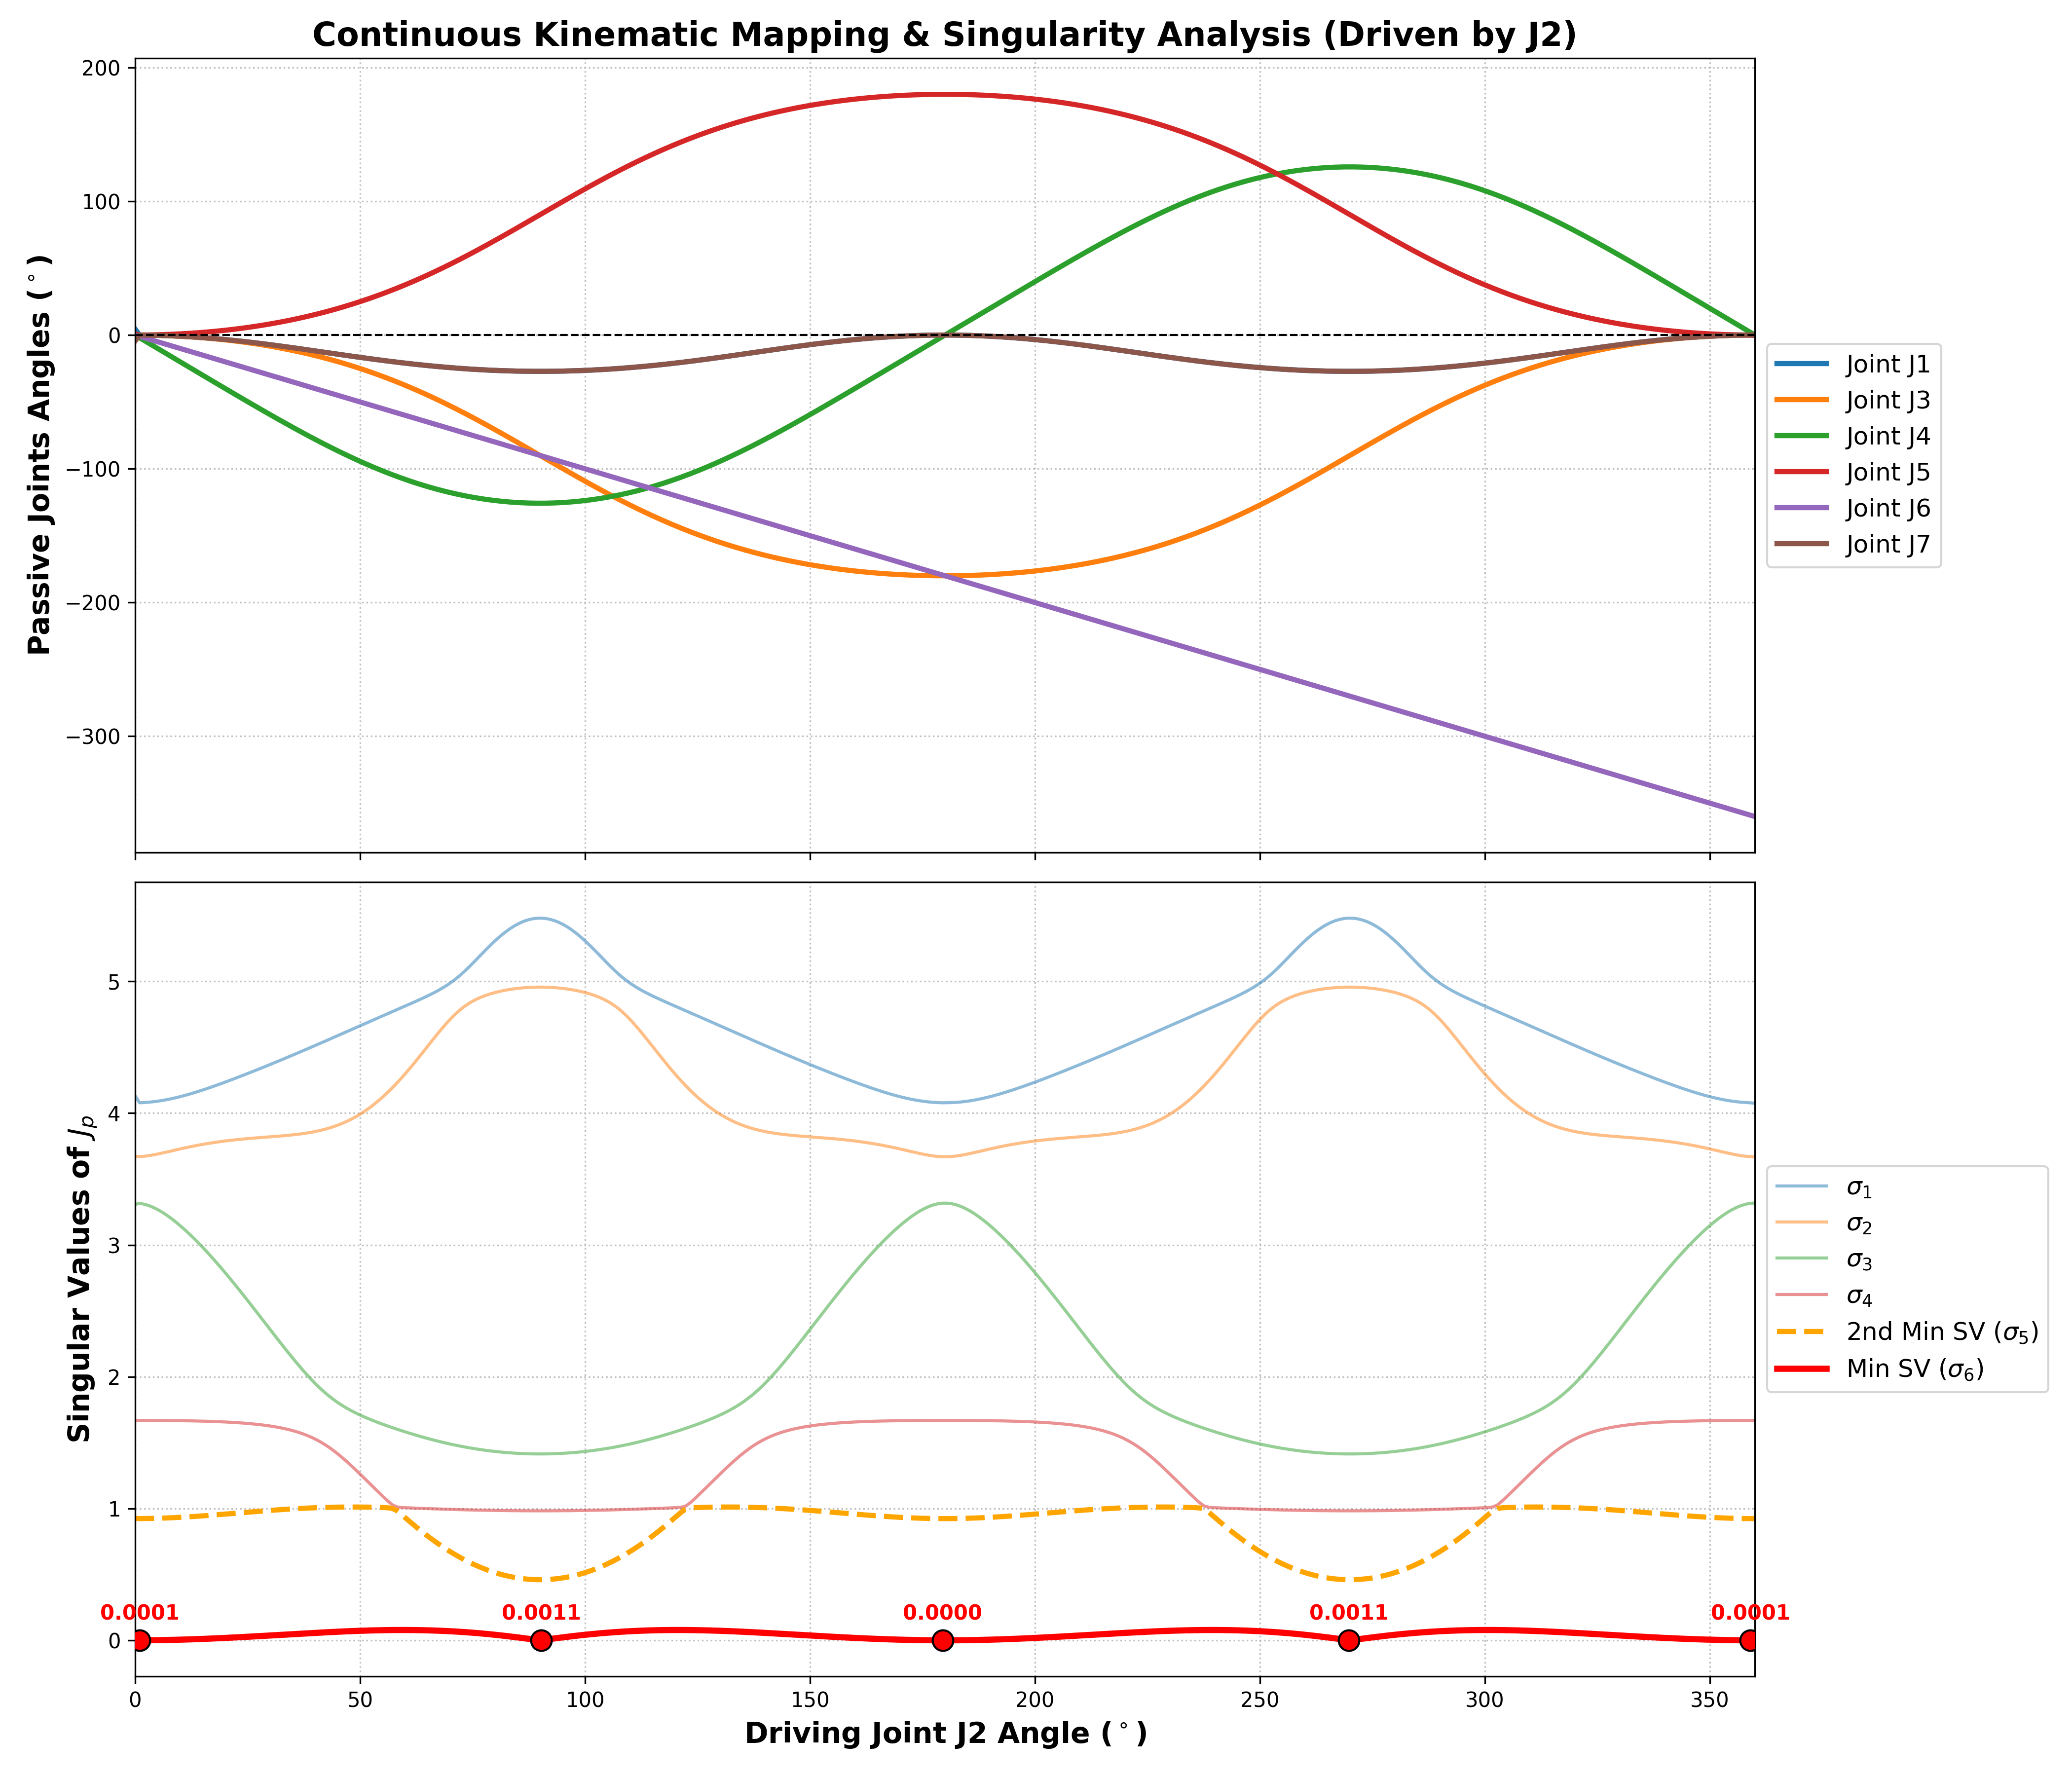
\includegraphics[width=1.0\textwidth]{j2_combined_analysis.png}
\caption{Continuous Kinematic Mapping \& Singularity Analysis}
\end{figure}

\section{Singularity Detection (Dead-center Points)}
In numerical computation, a singularity occurs when the minimum singular value ($\sigma_6$) of the passive Jacobian matrix approaches zero. By finding the local minima of $\sigma_6$, the following critical singular configurations (where $\sigma_6 < 0.1$) were identified:
\begin{itemize}
    \item Driving Joint $J_2 = 1.00^\circ$, Minimum Singular Value $\sigma_6 = 0.000108$
    \item Driving Joint $J_2 = 90.25^\circ$, Minimum Singular Value $\sigma_6 = 0.001138$
    \item Driving Joint $J_2 = 179.50^\circ$, Minimum Singular Value $\sigma_6 = 0.000024$
    \item Driving Joint $J_2 = 269.75^\circ$, Minimum Singular Value $\sigma_6 = 0.001138$
    \item Driving Joint $J_2 = 359.00^\circ$, Minimum Singular Value $\sigma_6 = 0.000098$
\end{itemize}

\section{Fourier Series Kinematic Mapping Formulas}
The discrete kinematic numerical solutions for the passive joints ($Q_i$ in degrees) driven by $J_2$ ($x$ in radians) have been fitted to 3rd-order Fourier series:
\begin{itemize}
    \item $J1(x) = -13.911 +0.023\cos(x) -0.000\sin(x) +13.665\cos(2x) -0.000\sin(2x) +0.023\cos(3x) -0.000\sin(3x)$
    \item $J3(x) = -89.997 +94.670\cos(x) -0.000\sin(x) +0.006\cos(2x) -0.000\sin(2x) -4.989\cos(3x) +0.000\sin(3x)$
    \item $J4(x) = -0.000 -0.000\cos(x) -124.037\sin(x) +0.000\cos(2x) -0.000\sin(2x) -0.000\cos(3x) +2.255\sin(3x)$
    \item $J5(x) = +90.001 -94.661\cos(x) -0.000\sin(x) +0.002\cos(2x) +0.000\sin(2x) +4.998\cos(3x) -0.000\sin(3x)$
    \item $J6(x) = -180.000 -0.000\cos(x) +114.589\sin(x) -0.000\cos(2x) +57.290\sin(2x) +0.000\cos(3x) +38.188\sin(3x)$
    \item $J7(x) = -13.933 -0.020\cos(x) +0.000\sin(x) +13.620\cos(2x) +0.000\sin(2x) -0.020\cos(3x) +0.000\sin(3x)$
\end{itemize}

\end{document}
